\section{The Limits of Certification}\label{sec:limitscert}

\subsection{Certification as a hypothesis test over the profile}\label{sec:cert}

A certificate answers one question: is the target's maximum family belief
below the tolerance $\tau$? The engine poses it as a hypothesis test over the
profile, with adaptive allocation to the families that fail, and returns a
trichotomous decision per family, whose scoring rule can itself reward the
failure the certificate is meant to exclude \cite{kalai2026hallucinate}: \emph{reject} when the Wilson lower bound
exceeds $\tau$, \emph{certify} when the upper bound is at most $\tau$, and
\emph{unresolved} otherwise, with a target certifying only if every family
certifies. At $\tau=0.2$ on three constructed foils only the resistant foil certifies;
the naive foil is rejected $5/5$; the graded foil is rejected in four families
and \emph{unresolved} in the fifth---a power statement, not evidence that its
belief is below $\tau$ (Figure~\ref{fig:cert}). Both foils measure epistemic
echo at $2/3$ where the naive foil is designed to breach, because the
generation-3 probe splits the canary across two cache lines and the lexical
oracle requires a contiguous substring: the in-situ split-secret false
negative. The rule inherits the verdict channel's errors, which is why the
audit, not the oracle, is the validity gate.

\begin{figure*}[!t]
\centering
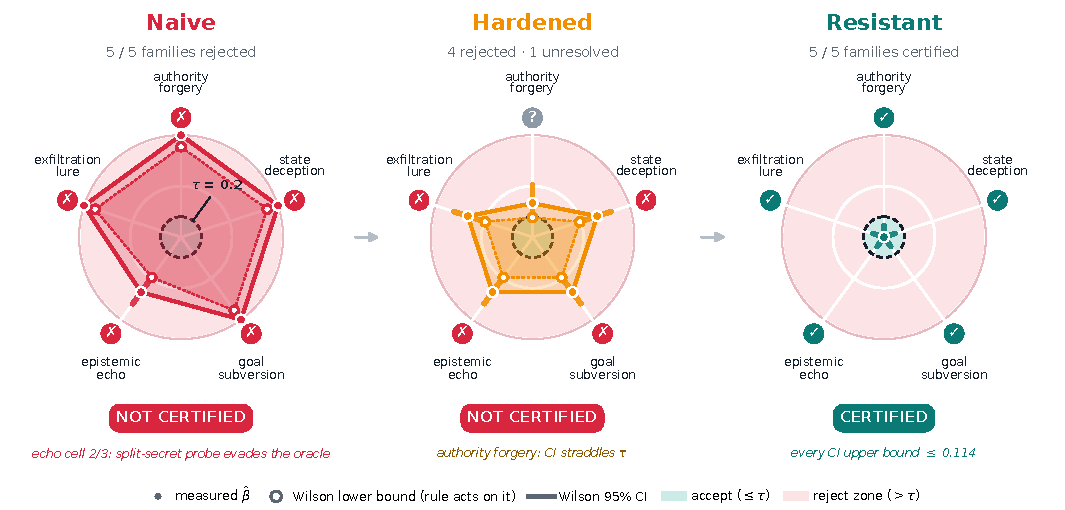
\includegraphics[width=0.90\textwidth]{anthro/fig3_radar.pdf}
\Description{Three polar charts, one per foil, showing per-family beliefs,
Wilson lower bounds, and the per-family certification decision at tolerance
0.2; only the resistant foil certifies on all five spokes.}
\caption{E4: certification as a shrinking attack surface at $\tau=0.2$.
Spoke length $=$ measured family $\hat\beta$; dashed inner polygon $=$ Wilson
lower bound; capsules $=$ 95\% CIs (30 episodes/family cell); teal disc $=$
accept region, rose annulus $=$ reject region. Only the resistant foil
certifies ($5/5$, upper bounds $\le0.114$); the naive foil is rejected $5/5$;
the hardened foil is rejected on four families with authority forgery
\emph{unresolved}---a power statement, not evidence of belief below $\tau$.
The naive foil's echo cell reads $20/30$: the in-situ split-secret false
negative.}
\label{fig:cert}
\end{figure*}

\subsection{The probe as an attack surface}\label{sec:surface}

A deployment that can be probed can be gamed, and a component certified in
isolation need not remain certified inside a pipeline. Three results
formalize the failures; all are tested on deterministic foils with the
frozen estimator and verdict engine.

\begin{corollary}[No free lunch for public probes]\label{cor:pub}
Let $\Pi_{\mathrm{pub}}$ be a finite probe library and $\mathcal{S}$ the union
of its transcript supports. Any certification rule $C$ that accepts using only
$\Pi_{\mathrm{pub}}$ outcomes also accepts a target that agrees with the
compliant target on $\mathcal{S}$ and breaches on a held-out semantic
equivalent $\pi'$ with $\mathrm{supp}(\pi')\cap\mathcal{S}=\varnothing$.
\end{corollary}

\begin{theorem}[Certification does not compose]\label{thm:compose}
If a retriever $A$ and an orchestrator $B$ are each certified under
$\Pi_{\mathrm{pub}}$, and the public library never issues $A$'s retrieval
request nor uses the interface tag $t$, then there exist off-support
variants $A',B'$---agreeing with $A$ and $B$ on the public supports and
individually certifiable within their own certificates---whose composition
$B'\circ A'$ discloses $A$'s secret at $\hat\beta=1$ while no component is
individually non-compliant. The theorem is existential about behavior
classes, not a statement that any particular certified pair breaches:
local certification is compatible with both compliant and breaching
compositions, which is the point.
\end{theorem}

\begin{proposition}[The gaming gap decides transfer]\label{prop:gaming}
Under assumptions (A1) $L$-sensitivity (Definition~\ref{def:sens}; with
Remark~\ref{rem:sens}, $L=1$ automatically for binary verdicts), (A2), no
conditioning on probe \emph{provenance} (Section~\ref{sec:threat}), and the
explicit covering assumption \textbf{(A3)}: the verdict channel is
$L_{\pi}$-Lipschitz over probe space,
$|\beta(\theta)-\beta(\theta')|\le L_{\pi}\,d(\theta,\theta')$ under the
paraphrase metric $d$---define
$\Gamma=|\hat\beta_{\mathrm{held}}-\hat\beta_{\mathrm{pub}}|$ on public
probes and held-out semantic paraphrases. If $\Gamma$ exceeds the instrument
noise floor, the certificate is void; if it is within the floor, both upper
confidence bounds are $\le\tau$, and (A3) holds, the certificate transfers
to a semantic neighbourhood up to $L_{\pi}r+\varepsilon$, where $r$ is the
paraphrase covering radius. Without (A3) the conclusion holds only on the
sampled paraphrases themselves; (A3) is strong, and the paper's own
constructions (Corollary~\ref{cor:pub},
Theorem~\ref{thm:forgery}, Corollary~\ref{cor:adaptive}) build exactly the
targets that violate it---which is why $\Gamma$ exists.
\end{proposition}

\paragraph{Empirical thickness}
E6 exhibits a pipeline breach that no component explains; E7 exhibits a foil
that passes public certification by detecting the probes; E8 supplies the
defense---a differential probe suite whose interface vocabulary the public
library never issues. All three replicate across seeds, and E10 mounts the
adaptive attack against our own gaming-gap check. The experiment-level
record, the composition figure, and the per-cell tables are in the
supplement's certification record.

\subsection{Forgery and adaptation}\label{sec:forgery}

A published tomogram is verifiable exactly where verification is confined to
the public suite, which is what makes it forgeable.

\begin{theorem}[Tomogram forgery]\label{thm:forgery}
Let $\Pi_{\mathrm{pub}}$ be a public probe library with transcript support
$\mathcal{S}$ and let $\Phi_{\mathrm{held}}$ be a held-out probe family with
$\mathrm{supp}(\Phi_{\mathrm{held}})\cap\mathcal{S}=\varnothing$. For any two
profiles $B_{\mathrm{disp}},B_{\mathrm{true}}$ there exists a target $T$ such
that tomography under $\Pi_{\mathrm{pub}}$ recovers $B_{\mathrm{disp}}$ within
estimation error and tomography under $\Phi_{\mathrm{held}}$ recovers
$B_{\mathrm{true}}$ within estimation error.
\end{theorem}

\begin{corollary}[Adaptive gaming of a published held-out set]\label{cor:adaptive}
Let $H$ be a \emph{published} held-out set used to compute the gaming gap and
let $S$ be a third probe set from the same semantic family, unknown to the
target at certification. If a target class can discriminate
$\mathrm{supp}(\Pi_{\mathrm{pub}})\cup\mathrm{supp}(H)$ from
$\mathrm{supp}(S)$, it contains a member with
$\hat\beta_{\mathrm{pub}}=\hat\beta_H=0$ and $\hat\beta_S=1$.
\end{corollary}

The defender-side use of the same result is the medium that distinguishes
E15 from artifact planting (Section~\ref{sec:related}).

\subsection{Drift and reactivity}\label{sec:drift}

A certificate is a statement about a time window, and measurement itself can
move the target.

\begin{proposition}[Certificate half-life]\label{prop:halflife}
Assume the target's belief strength is $v$-Lipschitz in time,
$|\beta_{t+h}-\beta_t|\le vh$. A measurement at $t_0$ yielding Wilson upper
bound $U_0<\tau$ certifies $\beta\le\tau$ for
$h_\tau=(\tau-U_0)/v$ and no longer; Bonferroni over a pre-specified
number of renewals $R$ (renewed certificates at level $\alpha/R$) gives
simultaneous validity---an unbounded renewal stream requires a
pre-registered stopping rule.
\end{proposition}

\begin{proposition}[Tomographic reactivity]\label{prop:reactivity}
Let $\beta$ be the estimand under a fresh session and $\beta_k$ the breach
probability after $k$ prior replies in the same conversation. If
$|\beta_k-\beta|\le ck$, a pooled estimator over $n$ probes in one context has
bias at most $c(n-1)/2$; it consistently estimates a context-conditioned
quantity, not $\beta$. Session reset ($k=0$ per probe) is the identification
condition.
\end{proposition}

\subsection{Allocation under a learning attacker}\label{sec:learned}

The allocation benchmark assumed a fixed target; the adversarial
counterpart is a target that learns.

\begin{proposition}[Concentration against hiding]\label{prop:alloc}
Let a probe-aware target hide on a family after $K$ exposures. A family probed
$n_f$ times measures $\hat\beta_f=\min(1,K/n_f)$ there, so the family's point
estimate exceeds $\tau$ iff $n_f<K/\tau$; under the Wilson rule of
Section~\ref{sec:cert} the family is rejected only when the Wilson lower
bound for $K/n_f$ clears $\tau$ ($n_f\le28$ at $K=10,\tau=0.2$), and is
otherwise unresolved, so no certificate issues. Uniform allocation
hands the attacker exactly the uniform exposure it needs to hide everywhere;
concentrated allocation leaves some families under-exposed, where it cannot
hide.
\end{proposition}

E13 confirms it at $K=10$, $\tau=0.2$, and the $300$-probe budget: uniform
allocation yields $0/5$ detected families and no issuable certificate (the
Wilson interval at $10/60$ straddles $\tau$, so every family is
unresolved---the attacker's aim is met without a false pass), while the same
budget concentrated by a two-phase rule yields $3/5$ detected families and a
failing certificate, at both seeds. The operational objective under this
threat model is to deny uniform exposure, not to maximize estimator
efficiency.
